\subsection{SCADA-системы}\label{par:scada}
\subsubsection{Что такое SCADA - система}
\Gls{scada} -- \glsdesc{scada} \cite{daneels_what_1999}.

Понятие SCADA - система включает в себя \cite{__2019}:
\begin{itemize}
	\item комплекс программ разработки ПО для обеспечения систем автоматизации;
	\item \Gls{pak} систем управления процессом, который осуществляет контроль и сбор данных.
\end{itemize}
\subsubsection{Задачи SCADA - систем}
Современная SCADA - система должна решать такие задачи, как \cite{daneels_what_1999, __2019, __2013-1}:
\begin{itemize}
	\item обмен данными с контроллерами, платами вывода и прочими устройствами (желательно в реальном времени);
	\item обработка полученной информации;
	\item отображение информации на \gls{mmi};
	\item ведение базы данных;
	\item аварийная сигнализация и управление тревожными сообщениями;
	\item связь с приложениями во внешней среде;
	\item автоматическое управление и корректирование в связи с изменением условий процесса;
	\item обеспечение оператора языком программирования для составления запросов к оборудованию;
	\item иметь в себе драйвера всех подключаемых устройств.
\end{itemize}
\subsubsection{Структура системы}
Структуру современной SCADA - системы можно описать так (см. \refris{fig:scadasys}): оборудование/датчики передают данные на ПЛК, которые отправляют данные оператору на \gls{mmi} (\glsdesc{mmi}).

\begin{figure}[p]
	\centering
	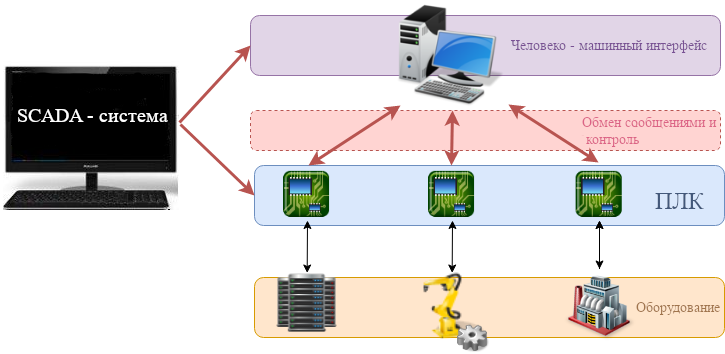
\includegraphics[width=\linewidth]{images/scadasys}
	\caption{Топология SCADA - системы}
	\label{fig:scadasys}
\end{figure}


\subsubsection{Пример применения SCADA систем}
SCADA - системы применяются во всех отраслях промышленности. На \refris{fig:at-genie} показана SCADA - система компании Advantech.


\begin{figure}[p]
	\centering
	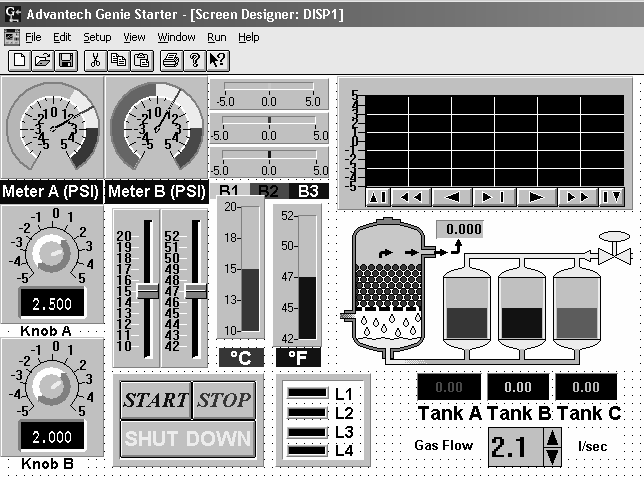
\includegraphics[width=\linewidth]{images/at-genie}
	\caption{SCADA - система Advantech Genie}
	\label{fig:at-genie}
\end{figure}

\subsection{Сравнение протоколов передачи данных промышленных сетей}
В \refpar{par:modbus}, \refpar{par:profibus} и \refpar{par:ffbus} были рассмотрены 3 протокола передачи данных для промышленных сетей.

Сравнение будет проводиться только среди \mb и \pb, поскольку хоть \ffb и является самым популярным протоколом с открытым стандартом и множеством возможностей, она не так широко распространена в мире и России, нет достаточной поддержки оборудования \cite{__2001, _foundation_1999}. 

\subsubsection{Modbus}
\noindent Особенности:
\begin{itemize}
	\item 3 разновидности: TCP, TRU и ACII;
	\item имеется контрольная сумма для проверки целостности;
	\item технология master - slave, только одно ведущее звено;
	\item максимум 32 устройства в сети (64 с повторителями).
\end{itemize}
Достоинства \cite{van_gorp_advanced_2009}:
\begin{itemize}
	\item хорошая документация;
	\item открытость;
	\item большое число поддерживаемых устройств.
\end{itemize}
Недостатки:
\begin{itemize}
	\item нет возможности диагностировать проблемы с устройствами, если такие случаются;
	\item некоторые производители могут добавить ``от себя'' и весь смысл стандартизации теряется.
\end{itemize}
\subsubsection{Profibus}
\noindent Особенности:
\begin{itemize}
	\item может иметь несколько ведущих звеньев, передающих важность при помощи маркера (см. \refpar{par:pb_work});
	\item имеется контрольная сумма для проверки целостности;
	\item технология master - slave;
	\item максимум 127 устройств;
	\item все устройства проходят сертификацию, поэтому совместимы без дополнительных ухищрений.
\end{itemize}
Достоинства:
\begin{itemize}
	\item поддержка цифрового и аналогового форматов;
	\item поддержка нескольких ведущих звеньев;
	\item простая масштабируемость и лёгкое добавление новых устройств.
\end{itemize}
Недостатки:
\begin{itemize}
	\item стандарт открыт не полностью (см. \cite{__2020});
	\item сложнее в освоении, чем \mb;
	\item в СНГ \mb более популярен.
\end{itemize}
\subsubsection{Итог}
Несмотря на все достоинства протокола \pb, описанные в \cite{powell_profibus_2013}, выбор пал на протокол \mb \tcp в связи с:
\begin{enumerate}
	\item Простой документацией;
	\item Полной открытостью;
	\item Наличием в современных средах разработки поддержки протокола \tcp (что облегчает работу с протоколом \mb \tcp);
	\item Оборудованием ОВЕН, работающем по протоколу \mb.
\end{enumerate}
\subsection{Примеры применения протокола Modbus для автоматизации}
Протокол применятся в разнообразных сферах деятельности человека:
\begin{enumerate}
	\item Передача показаний приборов учёта \cite{__2016};
	\item Автоматизация вакуумной установки \cite{__2017}. Исследование показало, что автоматизация установки минимизирует количество ошибок оператора, тем самым повышается надёжность процесса и облегчается работа оператора;
	\item Мониторинг теплиц, мониторинг системы нагрева воды солнечной энергией \cite{advantech__2019}.
\end{enumerate}
\subsection{Преимущества автоматизации}
К преимуществам автоматизации можно отнести:
\begin{itemize}
	\item уменьшение количества ошибок оператора;
	\item упрощение контроля за процессом;
	\item повышение надёжности процесса.
\end{itemize}
\subsection{Дальнейшая работа}
На основе проведённой научной работы и выбора протоколов передачи данных для автоматизации технологического процесса необходимо изучить одну из современных сред разработки, которая позволяет использовать все возможности протоколов \mb и \tcp.